\begin{columns}
  \begin{column}{0.35\textwidth}
    \begin{figure}
      \centering
      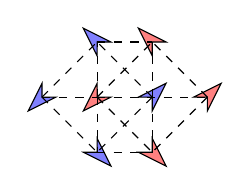
\begin{tikzpicture}[scale=0.7]
        \draw[fill=blue!50] (3,3) -- (2.75,3) -- (3.25,3.25) -- (3,2.75) -- cycle;
        \draw[fill=blue!50] (1,3) -- (1,3.25) -- (0.75,2.75) -- (1.25,3) -- cycle;
        \draw[fill=blue!50] (2.25,1.75) -- (2,2.25) -- (2,2) -- (1.75,2) -- cycle;
        \draw[fill=blue!50] (1.75,4.25) -- (2,3.75) -- (2,4) -- (2.25,4) -- cycle;
        \draw[dashed](1,3) -- (2,4);
        \draw[dashed](3,3) -- (2,4);
        \draw[dashed](3,3) -- (2,2);
        \draw[dashed](1,3) -- (2,2);
        \draw[fill=red!50] (4,3) -- (3.75,3) -- (4.25,3.25) -- (4,2.75) -- cycle;
        \draw[fill=red!50] (2,3) -- (2,3.25) -- (1.75,2.75) -- (2.25,3) -- cycle;
        \draw[fill=red!50] (3.25,1.75) -- (3,2.25) -- (3,2) -- (2.75,2) -- cycle;
        \draw[fill=red!50] (2.75,4.25) -- (3,3.75) -- (3,4) -- (3.25,4) -- cycle;
        \draw[dashed](2,3) -- (3,4);
        \draw[dashed](4,3) -- (3,4);
        \draw[dashed](4,3) -- (3,2);
        \draw[dashed](2,3) -- (3,2);
        \draw[dashed](2,3) -- (3,3);
        \draw[dashed](2,3) -- (2,4);
        \draw[dashed](2,3) -- (4,3);
        \draw[dashed](2,4) -- (3,4);
        \draw[dashed](3,3) -- (3,2);
        \draw[dashed](3,3) -- (3,4);
        \draw[dashed](2,3) -- (2,2);
        \draw[dashed](2,2) -- (3,2);
        \draw[dashed](1,3) -- (2,3);
      \end{tikzpicture}
      %\caption{The positions of the robots do not satisfy
       % the lattice graph A.}
    \end{figure}
  \end{column}
  \begin{column}{0.55\textwidth}
    \begin{figure}
      \centering
      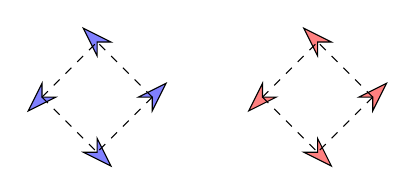
\begin{tikzpicture}[scale=0.7]
        \draw[fill=blue!50] (3,3) -- (2.75,3) -- (3.25,3.25) -- (3,2.75) -- cycle;
        \draw[fill=blue!50] (1,3) -- (1,3.25) -- (0.75,2.75) -- (1.25,3) -- cycle;
        \draw[fill=blue!50] (2.25,1.75) -- (2,2.25) -- (2,2) -- (1.75,2) -- cycle;
        \draw[fill=blue!50] (1.75,4.25) -- (2,3.75) -- (2,4) -- (2.25,4) -- cycle;
        \draw[dashed](1,3) -- (2,4);
        \draw[dashed](3,3) -- (2,4);
        \draw[dashed](3,3) -- (2,2);
        \draw[dashed](1,3) -- (2,2);
        \draw[fill=red!50] (7,3) -- (6.75,3) -- (7.25,3.25) -- (7,2.75) -- cycle;
        \draw[fill=red!50] (5,3) -- (5,3.25) -- (4.75,2.75) -- (5.25,3) -- cycle;
        \draw[fill=red!50] (6.25,1.75) -- (6,2.25) -- (6,2) -- (5.75,2) -- cycle;
        \draw[fill=red!50] (5.75,4.25) -- (6,3.75) -- (6,4) -- (6.25,4) -- cycle;
        \draw[dashed](5,3) -- (6,4);
        \draw[dashed](7,3) -- (6,4);
        \draw[dashed](7,3) -- (6,2);
        \draw[dashed](5,3) -- (6,2);
      \end{tikzpicture}
      %\caption{The positions of the robots satisfy the lattice graph A.}
    \end{figure}
  \end{column}
\end{columns}